\documentclass[12pt]{beamer}
\usepackage{tikz}
\usetikzlibrary{automata}
\usetheme{EastLansing}
\title{GRAPH THEORY PRESENTATION } 
\subtitle{Mathematics (582)}
  
\institute{Central Department of mathematics.}
\date{\today}
\begin{document}
\begin{frame}
\maketitle
\end{frame}

\begin{frame}[t]{Presenter Name lists}
\begin{itemize}
  \item 1 Durga Pokharel
  \item 2.Kamala Lm Magar
  \item 3.Sadhna Limbu
  \item 4.Lekhak chand
  \item 5.Jaylal shah
  \item 6.Dinesh Khanel
  \item 7.Shefequr Rehman 
  \item 8.Krishna Chaudhary
  \item 9.Dipesh Gurung
\end{itemize}
\end{frame}

\begin{frame}[t]{Contents}
\begin{enumerate}
\item Graph
\item Vertex
\item Arc
\item Directed graph
\item Undirected graph
\item Degree of digraph
\item Weighted Graphs
\item Isomorphism,Cartesian Product,Union

\end{enumerate}
\end{frame}
\begin{frame}[t]{Graph}
A graph is defined as G = (V , A). Where V is the set of vertices and A is the set of arcs.
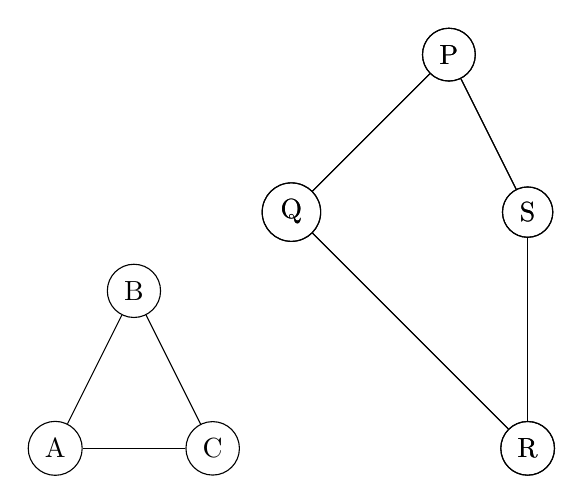
\begin{tikzpicture}
\node[circle ,draw=black](v1)at(5,5){P};
\node[circle,draw=black](v2) at (3,3){Q};
\node[circle,draw = black](v3) at(6,0) {R};
\node[circle,draw = black](v4) at(6,3){S};
\draw[-](v1)--(v2);
\draw[-](v2)--(v3);
\draw[-](v3)--(v4);
\draw[-](v4)--(v1);


\node[circle ,draw=black](v1)at(0,0){A};
\node[circle,draw=black](v2) at (1,2){B};
\node[circle,draw = black](v3) at(2,0) {C};

\draw[-](v1)--(v2);
\draw[-](v2)--(v3);
\draw[-](v3)--(v1);
\node[circle ,draw=black](v1)at(5,5){P};
\node[circle,draw=black](v2) at (3,3){Q};
\node[circle,draw = black](v3) at(6,0) {R};
\node[circle,draw = black](v4) at(6,3){S};
\draw[-](v1)--(v2);
\draw[-](v2)--(v3);
\draw[-](v3)--(v4);
\draw[-](v4)--(v1);
\end{tikzpicture}
\end{frame}
\begin{frame}[t]{Vertex}
The set of vertices or node is denoted by V(D).\\.
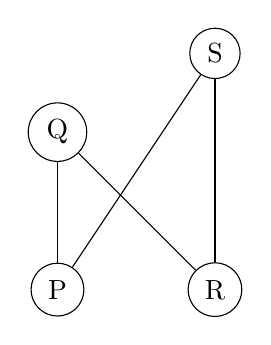
\begin{tikzpicture}
\node[circle ,draw=black](v1)at(0,0){P};
\node[circle,draw=black](v2) at (0,2){Q};
\node[circle,draw = black](v3) at(2,0) {R};
\node[circle,draw = black](v4) at(2,3){S};
\draw[-](v1)--(v2);
\draw[-](v2)--(v3);
\draw[-](v3)--(v4);
\draw[-](v4)--(v1);
\end{tikzpicture}\\
In above figure vertices are,\\
 V = \{P, Q, R, S\}\\
 Note:-Number of vertex are called degree of digraph.
\end{frame}
\begin{frame}[t]{Arcs}
The set of arcs are denoted by A(D).\\
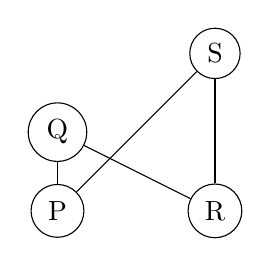
\begin{tikzpicture}
\node[circle ,draw=black](v1)at(0,0){P};
\node[circle,draw=black](v2) at (0,1){Q};
\node[circle,draw = black](v3) at(2,0) {R};
\node[circle,draw = black](v4) at(2,2){S};
\draw[-](v1)--(v2);
\draw[-](v2)--(v3);
\draw[-](v3)--(v4);
\draw[-](v4)--(v1);
\end{tikzpicture}\\
The arcs of above figure are,\\
A = \{(P, Q),(P, S),(S, R),(R, S)\}\\
Note: In above figure we can take any node as incident node as well as end node.\\
Note:-Number of arcs exists are called size of digraph.
\end{frame}
\begin{frame}[t]{Directed graph}
A graph is digraph if the arc(edge) are directed.\\
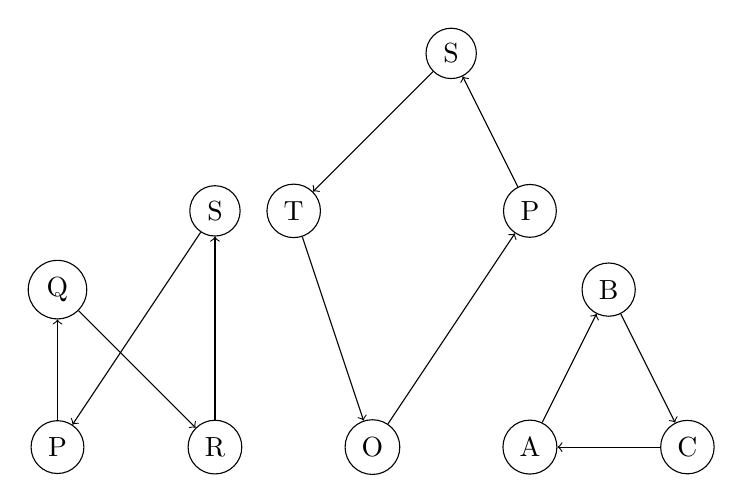
\begin{tikzpicture}
\node[circle ,draw=black](v1)at(0,0){P};
\node[circle,draw=black](v2) at (0,2){Q};
\node[circle,draw = black](v3) at(2,0) {R};
\node[circle,draw = black](v4) at(2,3){S};
\draw[->](v1)--(v2);
\draw[->](v2)--(v3);
\draw[->](v3)--(v4);
\draw[->](v4)--(v1);


\node[circle ,draw=black](v1)at(5,5){S};
\node[circle,draw=black](v2) at (3,3){T};
\node[circle,draw = black](v3) at(4,0) {O};
\node[circle,draw = black](v4) at(6,3){P};
\draw[->](v1)--(v2);
\draw[->](v2)--(v3);
\draw[->](v3)--(v4);
\draw[->](v4)--(v1);

\node[circle ,draw=black](v1)at(6,0){A};
\node[circle,draw=black](v2) at (7,2){B};
\node[circle,draw = black](v3) at(8,0) {C};
\draw[->](v1)--(v2);
\draw[->](v2)--(v3);
\draw[->](v3)--(v1);
\end{tikzpicture}
\end{frame}
\begin{frame}[t]
1. Tail.\\
2. Head.\\
3. End-nodes.\\
4. Adjacent arc.\\
5. Dominated vertex.

In figure PQRS tails are \{P ,Q ,R ,S\}and head are \{Q ,R ,S ,P\}.\\
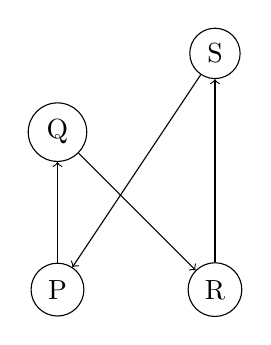
\begin{tikzpicture}
\node[circle ,draw=black](v1)at(0,0){P};
\node[circle,draw=black](v2) at (0,2){Q};
\node[circle,draw = black](v3) at(2,0) {R};
\node[circle,draw = black](v4) at(2,3){S};
\draw[->](v1)--(v2);
\draw[->](v2)--(v3);
\draw[->](v3)--(v4);
\draw[->](v4)--(v1);
\end{tikzpicture}
\end{frame}
\begin{frame}[t]{Undirected Graph}
If the arcs are not directed the graph is  undirected graph.\\
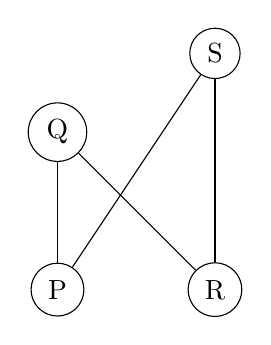
\begin{tikzpicture}
\node[circle,draw=black](v1)at(0,0){P};
\node[circle,draw=black](v2) at (0,2){Q};
\node[circle,draw = black](v3) at(2,0){R};
\node[circle,draw = black](v4) at(2,3){S};
\draw[-](v1)--(v2);
\draw[-](v2)--(v3);
\draw[-](v3)--(v4);
\draw[-](v4)--(v1);
\end{tikzpicture}\\
In above figure no arcs are directed from one vertex to another.\\

\end{frame}
\begin{frame}[t]{Types of Digraph}
\begin{itemize}
 \item Simple Digraph
 \item Parallel Digraph
 \item Multi Digraph
 \item Pseudo Digraph
\end{itemize}
1. Simple Digraph\\             
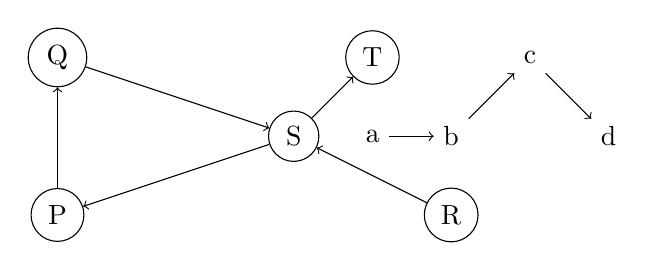
\begin{tikzpicture}
\node[circle,draw=black](v1)at(0,0){P};
\node[circle,draw=black](v2) at (0,2){Q};
\node[circle,draw = black](v3) at(5,0){R};
\node[circle,draw = black](v4) at(3,1){S};
\node[circle,draw = black](v5) at (4,2){T};
\draw[->](v1)--(v2);
\draw[->](v2)--(v4);
\draw[->](v3)--(v4);
\draw[->](v4)--(v1);
\draw[->](v4)--(v5);
\node[](v1)at(4,1){a};
\node[](v2) at (5,1){b};
\node[](v3) at(6,2) {c};
\node[](v4) at(7,1){d};
\draw[->](v1)--(v2);
\draw[->](v2)--(v3);
\draw[->](v3)--(v4);
\end{tikzpicture}
\end{frame}
\begin{frame}[t]
2. Parallel\\
\begin{tikzpicture}
\node[](v1)at(4,1){a};
\node[](v2) at (6,1){b};
\node[](v3) at(6,2) {c};
\node[](v4) at(7,1){d};
\node[](v5) at (8,1){e};
\node[](v6) at (9,0){f};
\draw[->](v1)--(v2);
\draw[->](v2)--(v3);
\draw[->](v3)--(v4);
\draw[->](v4)--(v5);
\draw[->](v5)--(v6);
\draw[->](v6)--(v5);
\draw[->](v1)edge[bend left](v2);

\node[](v1)at(0,0){P};
\node[](v2) at (0,2){Q};
\node[](v3) at(2,0){R};
\node[](v4) at(1,1){S};
\node[](v5) at (2,2){T};
\draw[->](v1)--(v2);
\draw[->](v2)--(v4);
\draw[->](v3)--(v4);
\draw[->](v4)--(v1);
\draw[->](v4)--(v5);
\draw[->](v5)--(v4);
\draw[->](v1)edge[bend left](v2);
\end{tikzpicture}\\
1. Loop.\\
2. Multiple arc.
\end{frame}
\begin{frame}[t]
3. Multi Digraph\\


\begin{tikzpicture}
\node[](v1)at(0,0){P};
\node[](v2) at (0,2){Q};
\node[](v3) at(2,3){R};
\node[](v4) at(3,3){S};
\draw[->](v1)--(v2);
\draw[->](v2)--(v3);
\draw[->](v3)--(v4);
\draw[->](v4)--(v1);
\draw[->](v1)--(v4);
\draw[->](v4)edge[bend left](v1);
\node[](v1)at(5,0){1};
\node[](v2) at (5,3){2};
\node[](v3) at(7,1){3};
\node[](v4) at(9,3){4};

\draw[->](v1)--(v2);
\draw[->](v2)--(v3);
\draw[->](v3)--(v4);

\draw[->](v4)edge[bend right](v3);
\end{tikzpicture}
\end{frame}
\begin{frame}[t]
4. Pseudo Digraph.\\
\begin{tikzpicture}
\node[](v1)at(0,0){w};
\node[](v2) at (0,2){x};
\node[](v3) at(5,0){y};
\node[](v4) at(3,1){z};
\node[](v5) at (4,2){v};
\draw[->](v1)--(v2);
\draw[->](v2)--(v4);
\draw[->](v3)--(v4);
\draw[->](v4)--(v1);
\draw[->](v4)--(v5);
\draw[->](v4)--(v4);
\draw[->](v2)--(v2);
\draw[->](v4)edge[loop](v4);
\node[](v1)at(6,3){1};
\node[](v2)at(7,4){2};
\node[](v3) at(7,0){3};
\draw[->](v1)--(v2);
\draw[->](v2)--(v3);
\draw[->](v3)--(v1);
\draw[->](v2)edge[loop](v2);
\end{tikzpicture}\\
1.Directed multi pseudograph.

\end{frame}
\begin{frame}[t]{Degree of Digraph}
1. Out-Degree\\
2. In-Degree\\

Degree\\
i. Minimum Simi-Degree\\
ii. Maximum Simi-Degree \\
iii. Regular Graph \\
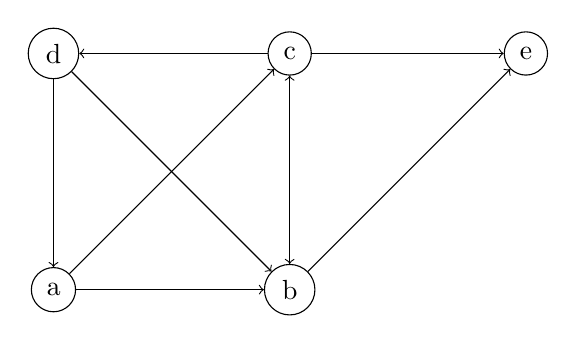
\begin{tikzpicture}
\node[circle ,draw=black](v1)at(0,0){a};
\node[circle,draw=black](v2) at (3,0){b};
\node[circle,draw = black](v3) at(3,3) {c};
\node[circle,draw = black](v4) at(0,3){d};
\node[circle,draw = black](v5) at(6,3){e};
\draw[->](v1)--(v2);
\draw[->](v2)--(v3);
\draw[->](v3)--(v4);
\draw[->](v4)--(v1);
\draw[->](v2)--(v5);
\draw[->](v3)--(v5);
\draw[->](v3)--(v2);
\draw[->](v4)--(v2);
\draw[->](v1)--(v3);
\end{tikzpicture}
\end{frame}
\begin{frame}[t]{Regular Digraph}

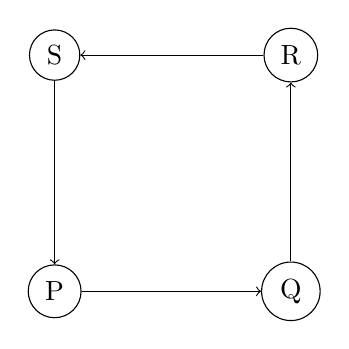
\begin{tikzpicture}
\node[circle ,draw=black](v1)at(0,0){P};
\node[circle,draw=black](v2) at (3,0){Q};
\node[circle,draw = black](v3) at(3,3) {R};
\node[circle,draw = black](v4) at(0,3){S};
\draw[->](v1)--(v2);
\draw[->](v2)--(v3);
\draw[->](v3)--(v4);
\draw[->](v4)--(v1);
\end{tikzpicture}\\
In above figure in-degree and out-degree are equal so it is example of regular digraph.
\end{frame}
\begin{frame}{Isomorphism}
        
	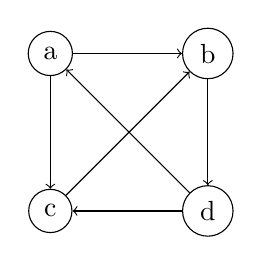
\begin{tikzpicture}
	\node[circle ,draw=black](v1)at(0,0){a};
	\node[circle,draw=black](v2) at (2,0){b};
	\node[circle,draw = black](v3) at(0,-2) {c};
	\node[circle,draw = black](v4) at(2,-2){d};
	\draw[->](v1)--(v2);
	\draw[<-](v2)--(v3);
	\draw[<-](v3)--(v4);
	\draw[->](v4)--(v1);
	\draw[->](v1)--(v3);
	\draw[->](v2)--(v4);
	\end{tikzpicture}
	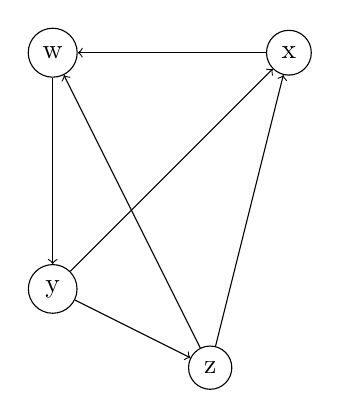
\begin{tikzpicture}
	\node[circle ,draw=black](v1)at(0,0){w};
	\node[circle,draw=black](v2) at (3,0){x};
	\node[circle,draw = black](v3) at(0,-3) {y};
	\node[circle,draw = black](v4) at(2,-4){z};
	\draw[<-](v1)--(v2);
	\draw[<-](v2)--(v3);
	\draw[->](v3)--(v4);
	\draw[->](v4)--(v1);
	\draw[->](v1)--(v3);
	\draw[<-](v2)--(v4);
	\end{tikzpicture}
	\end{frame}
\begin{frame}[t]{Cartesian Product}
Following are two figures first (A) and second figure is (B)\\

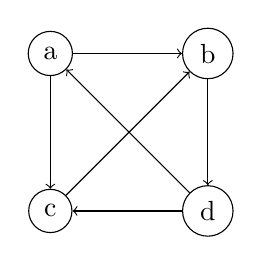
\begin{tikzpicture}
\node[circle ,draw=black](v1)at(0,0){a};
\node[circle,draw=black](v2) at (2,0){b};
\node[circle,draw = black](v3) at(0,-2) {c};
\node[circle,draw = black](v4) at(2,-2){d};
\draw[->](v1)--(v2);
\draw[<-](v2)--(v3);
\draw[<-](v3)--(v4);
\draw[->](v4)--(v1);
\draw[->](v1)--(v3);
\draw[->](v2)--(v4);
\end{tikzpicture}
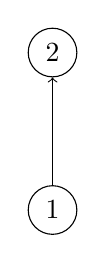
\begin{tikzpicture}
\node[circle ,draw=black](v1)at(2,2){2};
\node[circle,draw=black](v2) at (2,0){1};
\draw[->](v2)--(v1);
\end{tikzpicture}
\end{frame}
\begin{frame}
Cartesian Product of figure(A) and (B) are displayed below.\\
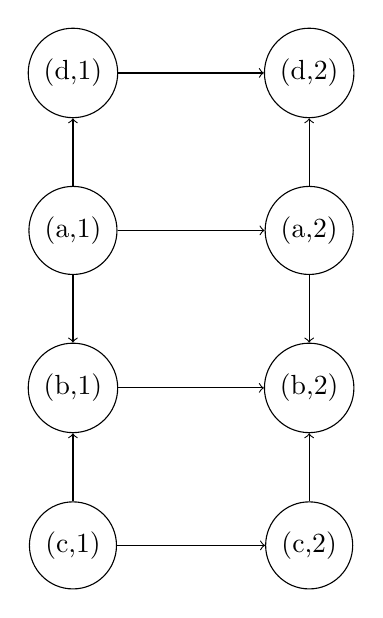
\begin{tikzpicture}
\node[circle ,draw=black](v1)at(0,0){(a,1)};
\node[circle,draw=black](v2) at (3,0){(a,2)};
\node[circle,draw = black](v3) at(0,-2) {(b,1)};
\node[circle,draw = black](v4) at(3,-2){(b,2)};
\node[circle,draw=black] (v5) at (0,-4){(c,1)};
\node[circle, draw= black] (v6) at (3,-4) {(c,2)};
\node[circle, draw = black] (v7) at (0,2) {(d,1)};
\node[circle, draw = black] (v8) at (3,2) {(d,2)};
\draw[->](v1)--(v2);
\draw[->](v1)--(v3);
\draw[->](v3)--(v4);
\draw[->](v2)--(v4);
\draw[->](v5)--(v6);
\draw[->](v5)--(v3);
\draw[->](v6)--(v4);
\draw[->](v7)--(v8);
\draw[->](v1)--(v7);
\draw[->](v2)--(v8);
\end{tikzpicture} 

\end {frame}
\begin{frame}[t]{Power of Digraph}
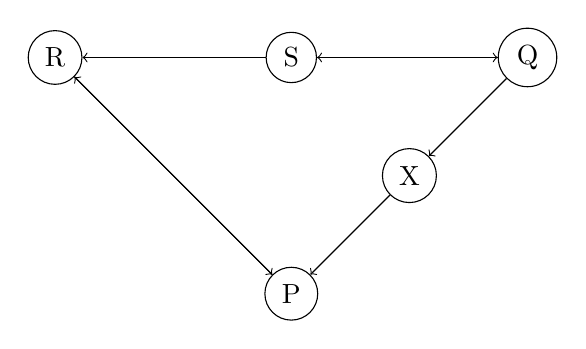
\begin{tikzpicture}
\node[circle,draw = black](v1)at(0,0){P};
\node[circle,draw = black](v2) at (3,3){Q};
\node[circle,draw = black](v3) at(-3,3) {R};
\node[circle,draw = black](v4) at(0,3){S};
\node[circle,draw = black](v5) at(1.5,1.5){X};
\draw[->](v1)--(v3);
\draw[->](v2)--(v4);
\draw[->](v2)--(v5);
\draw[->](v3)--(v1);
\draw[->](v4)--(v3);
\draw[->](v4)--(v2);
\draw[->](v5)--(v1);
\end{tikzpicture}
\end{frame}
\begin{frame}[t]
If we take p = 2 then we see following figure.\\
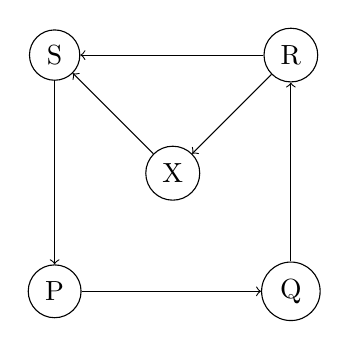
\begin{tikzpicture}
\node[circle,draw = black](v1)at(0,0){P};
\node[circle,draw = black](v2) at (3,0){Q};
\node[circle,draw = black](v3) at(3,3) {R};
\node[circle,draw = black](v4) at(0,3){S};
\node[circle,draw = black](v5) at(1.5,1.5){X};
\draw[->](v1)--(v2);
\draw[->](v2)--(v3);
\draw[->](v3)--(v4);
\draw[->](v4)--(v1);
\draw[->](v5)--(v4);
\draw[->](v3)--(v5);
\end{tikzpicture}
\end{frame}
\begin{frame}[t]{Union of Two Digraph}
Digraph H,\\
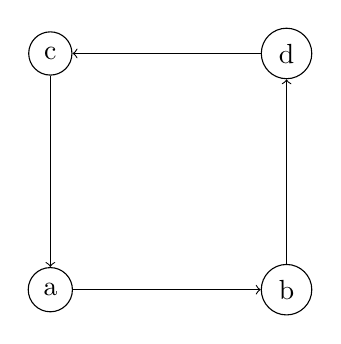
\begin{tikzpicture}
\node[circle,draw = black](v1)at(0,0){a};
\node[circle,draw = black](v2) at (3,0){b};
\node[circle,draw = black](v3) at(3,3) {d};
\node[circle,draw = black](v4) at(0,3){c};

\draw[->](v1)--(v2);
\draw[->](v2)--(v3);
\draw[->](v3)--(v4);
\draw[->](v4)--(v1);
\end{tikzpicture}
\end{frame}
\begin{frame}[t]
Digraph L.\\
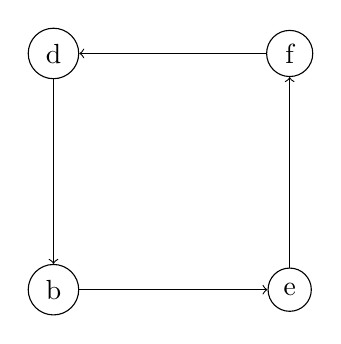
\begin{tikzpicture}
\node[circle,draw = black](v1)at(0,0){b};
\node[circle,draw = black](v2) at (3,0){e};
\node[circle,draw = black](v3) at(3,3) {f};
\node[circle,draw = black](v4) at(0,3){d};
\draw[->](v1)--(v2);
\draw[->](v2)--(v3);
\draw[->](v3)--(v4);
\draw[->](v4)--(v1);
\end{tikzpicture}
\end{frame}
\begin{frame}[t]
Union of H and L  displayed below.\\
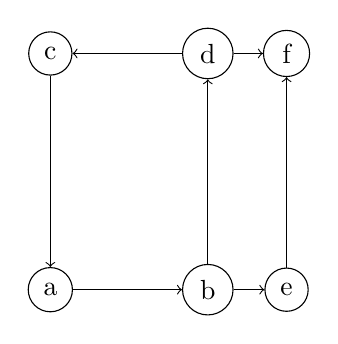
\begin{tikzpicture}
\node[circle,draw = black](v1)at(0,0){a};
\node[circle,draw = black](v2) at (2,0){b};
\node[circle,draw = black](v3) at(3,0) {e};
\node[circle,draw = black](v4) at(0,3){c};
\node[circle,draw = black](v5) at(2,3){d};
\node[circle,draw = black](v6) at(3,3){f};
\draw[->](v1)--(v2);
\draw[->](v2)--(v3);

\draw[->](v4)--(v1);
\draw[->](v2)--(v5);
\draw[->](v5)--(v4);
\draw[->](v5)--(v6);
\draw[->](v3)--(v6);
\end{tikzpicture}
\end{frame}

\end{document}
 
